\documentclass[a4paper]{article}

% Includes packages relevant to Senior Lab

% character set specifications
\usepackage[english]{babel}
\usepackage[utf8]{inputenc}

% increased vertical spacing for tables
\newcommand\topVspace{\rule{0pt}{2.6ex}}      
\newcommand\bottomVspace{\rule[-1.2ex]{0pt}{0pt}} 

% extra unicode characters
\DeclareUnicodeCharacter{3BC}{\(\mu\)}
\DeclareUnicodeCharacter{3C1}{\(\rho\)}
\DeclareUnicodeCharacter{2080}{\(_0\)}
\DeclareUnicodeCharacter{2081}{\(_1\)}
\DeclareUnicodeCharacter{2082}{\(_2\)}
\DeclareUnicodeCharacter{3B5}{\(\epsilon\)}
\DeclareUnicodeCharacter{3B1}{\(\alpha\)}

% SI Units
\usepackage{siunitx}

% extra SI units
\DeclareSIUnit\gauss{G}

% enable scientific notation
\sisetup{scientific-notation = engineering, exponent-to-prefix}

% draw pretty lines
\usepackage{tikz}
\usetikzlibrary{datavisualization}
\usepackage{circuitikz}

% manual tabbing
\setlength{\parindent}{0pt}
\def\qq{\qquad}

% include graphics
\usepackage{graphicx}

% increased control over figure placement
\usepackage{float}

% box answers
\usepackage{tcolorbox}

% enable multiple section levels
\usepackage{titlesec}

% define `\subsubsubsection` command
\titleclass{\subsubsubsection}{straight}[\subsection]
\newcounter{subsubsubsection}[subsubsection]
\renewcommand\thesubsubsubsection{\thesubsubsection.\arabic{subsubsubsection}}
\titleformat{\subsubsubsection}
        {\normalfont\normalsize\bfseries}{\thesubsubsubsection}{1em}{}
\titlespacing*{\subsubsubsection}
{0pt}{3.25ex plus 1ex minus .2ex}{1.5ex plus .2ex}
\setcounter{secnumdepth}{4}

% get align environment (among other things)
\usepackage{amsmath}

% bold in math mode
\usepackage{bm}

% get \mathbb (among other things)
\usepackage{amssymb}

\usepackage{array}

% plotting
\usepackage{pgfplots}

% enable external references
\usepackage{hyperref}

% include code
\usepackage[cache=false]{minted}
\setminted{linenos, frame=lines, texcomments}

% adjust margins of individual pages (for shoving figures into place)
\usepackage{changepage}

% rotate figures
\usepackage{rotating}


\usepackage{caption}
\renewcommand{\thetable}{\arabic{section}.\arabic{table}}
\newcommand\T{\rule{0pt}{2.6ex}}       % Top strut
\newcommand\B{\rule[-1.2ex]{0pt}{0pt}} % Bottom strut

\title{PHY 4210-01 Senior Lab \\Lab N4: Rutherford Scattering}

\author{Sarah Arends \\ 
        Jacquelyne Miksanek \\
        Ryan Wojtyla \\ \\
        Instructor: Dr. Marcus Hohlmann}

\date{March 14, 2019}

\begin{document}
\maketitle 

\begin{abstract}
%physics of experiment
%apparatus used
%what was measured
%Results
  \qq 
\end{abstract}

\newpage

\tableofcontents

\newpage

\section{Objective of the Experiment}
%A brief statement on the main purpose of the experiment
\qq 

\section{Theory of the Experiment}
%A short presentation of the concepts and formulas related to the experiment. 

% How Rutherford scattering works (Coulomb repulsion etc)
\qq

% Physical meaning and derivation of differential cross section
\qq When an alpha particle with impact parameter \( b \) approaches a nucleus,
it is scattered at an angle \( \theta \). If the impact parameter is given an
infinitesimal range of [ \( b \), \( b + db \) ], the resulting scattering angle
then has a range of [ \( \theta - d\theta \), \( \theta \) ]; the impact
parameter and scattering angle are inversely proportional. 

\qq Because the alpha particle can be incident within a defined range at any
angle relative to the nucleus, a ring of possible incident locations is created
in front of the nucleus. This ring is illustrated in Figure
\ref{fig:crossSecRing}.

\begin{figure}[H]
  \begin{center}
    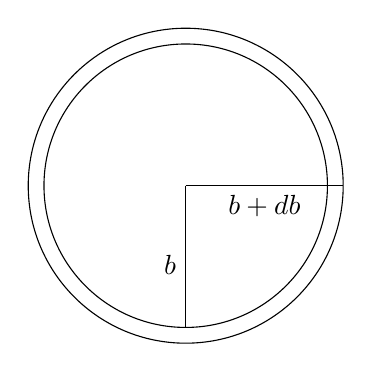
\begin{tikzpicture}
      \draw (0,0) circle [radius=2.0];
      \draw (0,0) circle [radius=1.8];
      \draw (0,0) -- (1,0) node[anchor=north] {\( b + db \)} -- (2,0);
      \draw (0,0) -- (0,-1.0) node[anchor=east] {\( b \)} -- (0,-1.8);
    \end{tikzpicture}
  \end{center}
  \caption{The ring whose area represents the possible region in which alpha
    particles may be incident on a target nucleus.}
  \label{fig:crossSecRing}
\end{figure}

The area of this ring is found as the area of any ring is found:

\begin{align*}
  A &= \pi (b + db)^2 - \pi b^2 \\
    &= \pi (b^2 + 2 b db + db^2) - \pi b^2 \\
    &= \pi b^2 + 2 \pi b db + \pi db^2 - \pi b^2 \\
    &= 2 \pi b db + \pi db^2 \\
\end{align*}

Since \( db \) is infinitesimally small, it can be approximated to be
zero. Therefore, the area of the incident ring, \( \Delta \sigma \), is

\begin{equation*}
  \Delta \sigma = 2 \pi b db
\end{equation*}

\qq Since \( \Delta \sigma \) is the area of the full incident ring, an
infinitesimal angular portion of that ring, \( d\phi \), may be represented by
\( \Delta \sigma (\phi) = b db d\phi \). Additionally, because the impact
parameter \( b \) is related to the scattering angle \( \theta \), \( \Delta
\sigma \) is also a function of \( \theta \). Hence, 

\begin{equation*}
  \Delta \sigma (\theta, \phi) = b db d\phi
\end{equation*}

\qq Since the impact parameter \( b \) is directly proportional to the size of
the cross section and the scattering angle \( \theta \) is inversely
proportional to the impact parameter, the size of the cross section decreases as
the scattering angle increases. Therefore, the cross section experiences a
negative rate of change as \( \theta \) increases. Hence, 

\begin{equation}
  \Delta \sigma (\theta, \phi) = - d\sigma (\theta, \phi) 
\end{equation}
\label{eqn:dSigma}

\qq 

\section{Equipment Utilized}
%List principal pieces of apparatus used by manufacturer, model and serial number. When it may be important, list principal specifications of certain pieces of equipment (e.g. the focal length of an optical system, etc.)

% Description of set-up in prose
\qq 

% List of specs
\begin{itemize}
\item List equipment and specifications
\end{itemize}

%Labeled sketch of the experimental setup
\begin{figure}[H]
\centering
% uncomment the line below to add image
%\includegraphics[width=0.5\textwidth]{figure.png}
\captionof{figure}{Description of schematic here}
\label{name}
\end{figure}

\section{Procedure}

% Describe the main steps in the experimental procedures. Be sure to include any
% precautions. Sufficient details should be given such that another student can
% follow and do the experiment.
\qq

\subsection{Procedural Modifications}

\qq 

\section{Data Analysis}

\subsection{Data Analysis I: Gold}
%Graphs, figures, and tables with captions
%Results with error analysis
%Calculate discrepancies from theory

% Direct counting rate as a function of angle (gold)
\qq

% Corrected counting rate (wrt. distribution in space)
\qq 

% Experimental results for rutherford formula
\qq 

% Experimental uncertainty (\delta)
\qq 

% Theoretical results for rutherford formula
\qq 

\subsection{Data Analysis II: Aluminum}
%Graphs, figures, and tables with captions
%Results with error analysis
%Calculate discrepancies from theory

% Direct counting rate as a function of angle (gold)
\qq

% Corrected counting rate (wrt. distribution in space)
\qq 

% Experimental results for rutherford formula
\qq 

% Experimental uncertainty (\delta)
\qq 

% Theoretical results for rutherford formula
\qq 

\section{Results}

\subsection{Results I: Gold}
%Discuss results and uncertainties
%Compare results with theory
%Approximations to theory

% Tabulate theo and exp values/uncertainties
\qq 

% Calculate the difference/discrepancy (\Delta)
\qq 

% Calculate the uncertainty in the discrepancy
% Quantify how many sigmas the discrepancy is
\qq

\subsection{Results II: Aluminum}
%Discuss results and uncertainties
%Compare results with theory
%Approximations to theory

% Tabulate theo and exp values/uncertainties
\qq 

% Calculate the difference/discrepancy (\Delta)
\qq 

% Calculate the uncertainty in the discrepancy
% Quantify how many sigmas the discrepancy is
\qq

\section{Conclusion}
%Brief summary, discussion of theory

% Results for gold
% Note the number of sigmas (discrepancy) and what that means statistically
\qq 

% Results for aluminum
% Note the number of sigmas (discrepancy) and what that means statistically
\qq 

\section{Appendices}

\subsection{Appendix A: Data}

\subsection{Appendix B: Source Code}

\end{document}
